\section{Experiments}

In this section, we present our findings from a set of performance experiments that we ran to test the scalability characteristics of Databus. 

\subsection{Experimental setup}

We ran our experiments on two types of machines:

\begin{itemize}
\item Relays and client machines - 12 core 2.56GHz Intel Xeon machines with 48 GB RAM, 1TB SATA RAID 1+0 and 1 Gbps Ethernet
\item Bootstrap servers - 12 core 2.40GHz Intel Xeon machines with 48 GB RAM, 800GB 15K SAS RAID 1+0 and 1 Gbps Ethernet
\end{itemize}

There were three main parameters that we varied:

\begin{itemize}
\item Event rate - the rate at which change events are being fetched into the relay buffer
\item Number of consumers - the number of applications that consume events from the relays and bootstrap service
\item Consumer poll interval - the frequency with which consumers poll the relays for new events
\end{itemize}

For all experiments, we used moderately-sized events with a size of 2.5KB.

The metrics we measured were

\begin{itemize}
\item Throughput - the number of events or bytes per second that the relay can push out to the consumers
\item E2E event latency - the time it takes for an event to propagate from the relay to the consumers
\end{itemize}

\subsection{Relay}

Figure \ref{fig:relay_throughput} shows the first set of experiments where we measured the maximum relay throughput and CPU utilization with different sets of consumers. We used a relay with already pre-filled buffers and measured the maximum speed at which multiple consumers can read from the relay. We varied the number of consumers and the consumer poll interval. The latter parameter allowed us to test the impact of polling less frequently but in bigger batches of events. We expected that less frequent but bigger batches would allow the relay to support larger number of consumers. The data series prefixed with ``tpt'' show the relay throughput in MB/s (e.g. ``tpt\_10'' shows the throughput for consumers using 10ms poll interval) with throughput being plotted on the left-hand side ``y'' axis. The data series prefixed with ``cpu'' show the relay CPU utilization percentage (e.g. ``cpu\_55'' shows the throughput for consumers using 55 ms poll interval) with the CPU utilization being plotted on the right-hand side ``y'' axis.

\begin{figure}
\centering
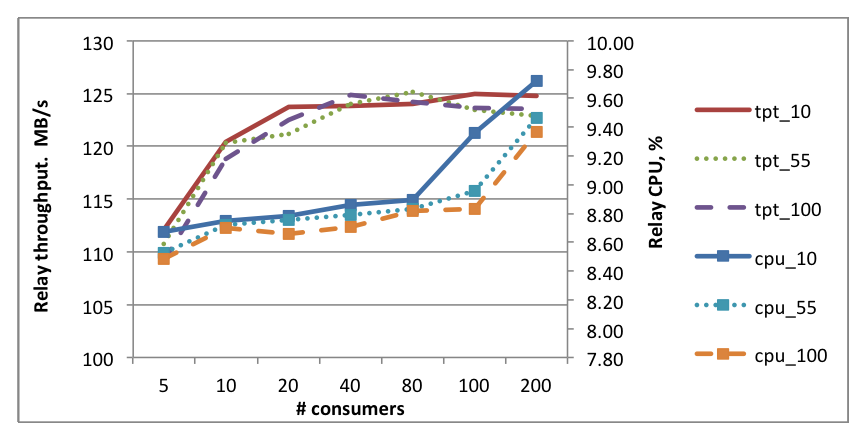
\epsfig{file=figures/relay_throughput.eps, width=3in}
\caption{Relay throughput scalability depending on poll interval}
\label{fig:relay_throughput}
\end{figure}

The experiments confirmed our hypothesis. With low poll intervals and fast processing consumers (as the ones that we used for our experiments), we can quickly saturate network bandwidth. We notice that once we get closer to network saturation, the relays do not scale linearly: doubling the number of consumers from 5 to 10 causes an increase of throughput of only 9\% (from 110MB/s to 120MB/s). We attribute this to networking overhead. The number of transmitted packets peaked at around 82 thousand packets/s even for 5 consumers and it did not increase with the number of consumers. Thus, increased number of consumers just leads to slightly better utilization of those packets.

Increasing the poll interval has only a small impact on the relay in terms of CPU utilization for small number of consumers. With increased number of consumers the effect becomes more pronounced although still the CPU utilization is fairly low -- less than 10\%. Overall, the experiments show that network bandwidth becomes a bottleneck much before the CPU. Thus, trading CPU for network bandwidth on the relay side can be expected to pay off. This is further explored in the experiments below.

The second set of experiments aimed at testing how writes to the relay buffer affected throughput. For this set of experiments, we gradually increased the update rate (100 update/s, 1000 updates/s, 2000 update/s) at the data source and measured the consumption throughput (in updates/s) and E2E latency (in milliseconds) at the consumers. Our goal was to detect when bottlenecks on the relay cause the consumers to fall behind the stream of updates from the data sources. We fixed the consumer poll interval at 10ms. Therefore, the consumers can expect on average 5 ms latency due to the poll frequency.   

Figure \ref{fig:throughput-poll10} shows the rate at which the consumers were receiving the events. For an event rate of 100 updates/s, the consumption rate stays flat at 100 updates/s, i.e. the consumers are keeping up with the update rate. For event rates of 1000 and 2000 updates/s, we observe two ``knees'' in the consumption rate when the number of consumers goes above 40 and 20 consumers respectively. These are the points at which the consumers are no longer able to keep up with the update stream. This behavior can again be explained by network bandwidth saturation: 40 consumers at 1000 updates/s utilize 100MB/s, close to the maximum network bandwidth. 

\begin{figure}
\centering
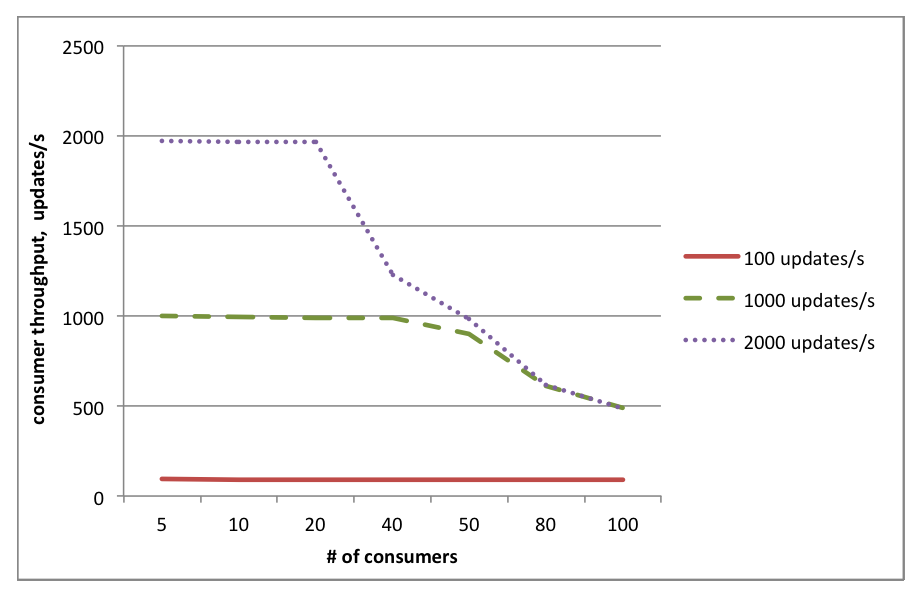
\epsfig{file=figures/consumer_throughput.eps, width=3in}
\caption{Throughput at consumers when varying update rate}
\label{fig:throughput-poll10}
\end{figure}

We observe a similar pattern when studying the E2E event latency on Figure~\ref{fig:latency-poll10}. At 100 updates/s, the E2E latency (including the poll interval) increases from 10ms to 20ms as the number of consumers grew. For 1000 and 2000 updates/s, we observe similar ``knees'' as the previous graph at 40 and 20 consumers. Up until those thresholds the E2E latency stays between 15 and 20ms and increases without recovery after that. 

\begin{figure}
\centering
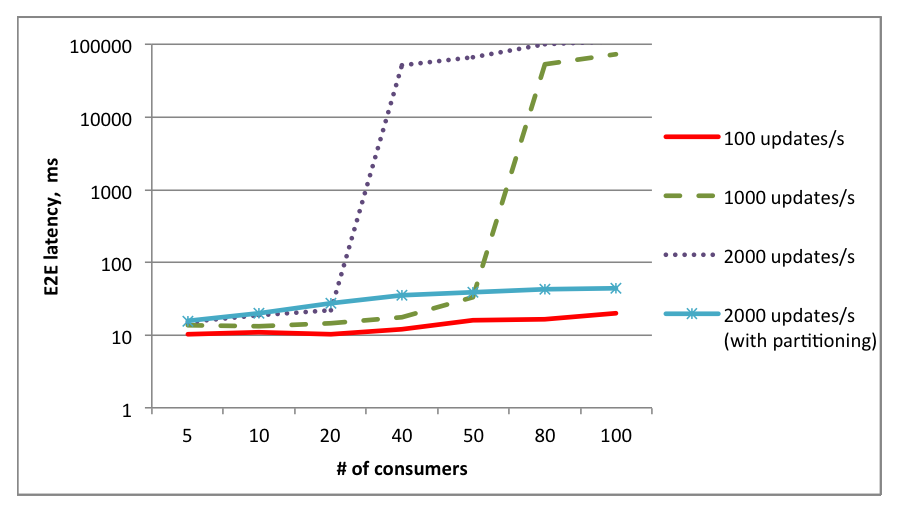
\epsfig{file=figures/e2e_latency.eps, width=3in}
\caption{Latency to consumers}
\label{fig:latency-poll10}
\end{figure}

For the experiment on Figure~\ref{fig:latency-poll10}, we also tested the effect of consumer partitioning using server-side filtering; each consumer only subscribes to a portion of the change stream. We wanted to remove the outbound network bandwidth bottleneck and see if the relay can scale to more consumers. The results are shown in the ``2000 updates/s (with partitioning)'' data series. For the experiment, we used a simple partitioning scheme where the key space is uniformly partitioned among all available consumers (a fairly typical scenario). In this case, the required outbound bandwidth is equal to the incoming data bandwidth and does not vary with the number of consumers. Although the E2E latency went up to a range of 15 to 45ms due to the additional server-side processing, the rate of increase in E2E latency is very gradual. Thus, we can conclude that the relay can scale to hundreds of consumers if the client application can tolerate slightly higher E2E latency.


\subsection{Bootstrap service}

We decided to setup our bootstrap performance experiments differently than our relay performance experiments. Firstly, the E2E latency metric used in the latter is not meaningful since the bootstrap service by definition serves older change records. Secondly, our initial bootstrap experiments showed that bootstrap servers can easily saturate the network bandwidth when bootstrapping multiple consumers, similarly to the relay experiments.

Instead, we focused on the more interesting aspect of the bootstrap service: the ability to serve compacted deltas of events from the snapshot store versus replaying all updates from the log store. 
On the one hand, serving from the log store utilizes very efficient sequential disk reads but has to return all change records. 
On the other hand, serving from the snapshot store allows the bootstrap service to stream out fewer records (because only the latest change record for a given key is returned) at the cost of a less efficient disk access pattern. 

The goal of our experiments was to find the break even point for the two access patterns. This helps us tune the retention policy in the bootstrap service and to implement an optimization in the bootstrap service where the snapshot phase can be bypassed if it is more beneficial to serve the bootstrap data entirely from the bootstrap log store. Thus, we introduced a new parameter: the ratio between updates to existing keys (including deletes) versus the total number of change records. This parameter models the benefit of returning only the latest version of the value for a given key. 

The experiments compared the time (in milliseconds) to do a full bootstrap on a set of test databases for which we varied the above ratio. We tested databases where the ratio varied from around 33\% to 99\%. The results are presented on Figure~\ref{fig:snapshot_vs_catchup}. 

\begin{figure}
\centering
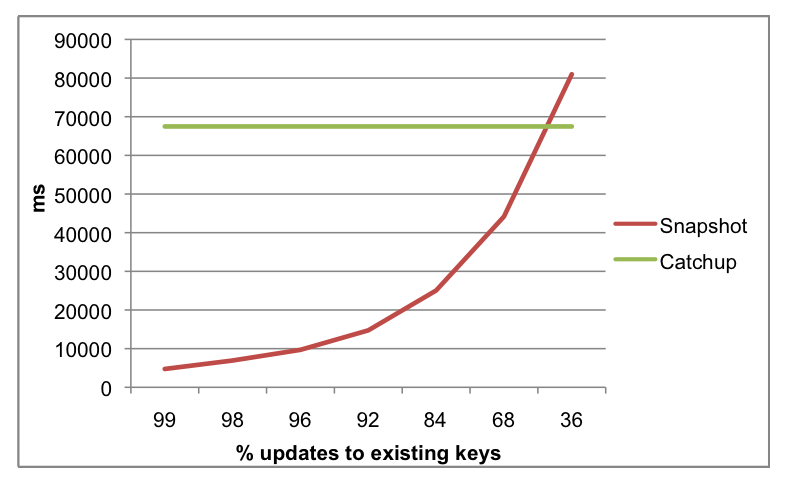
\epsfig{file=figures/snapshot_vs_catchup.eps, width=3in}
\caption{Time to bootstrap 1 hour of changes using a Snapshot delta or Catch-up log}
\label{fig:snapshot_vs_catchup}
\end{figure}

Our experiments show that with maintaining the appropriate index structures on the snapshot store, returning compacted deltas from the snapshot store is very efficient. The break-even point is when about half of the change records contain updates to existing keys. In practice, we actively monitor the above ratio in production and use the results from these experiments to tune our bootstrap services. Since the ratio changes slowly, the configuration is manual. In the future, we plan to make the bootstrap service auto-tunable.



